\documentclass[a4paper,12pt]{article}
\usepackage[utf8]{inputenc}
\usepackage[french]{babel}
\usepackage[T1]{fontenc}
\usepackage{graphicx}
\begin{document}
\begin{titlepage}

\begin{flushleft}
GORON Nathan 21503237
\newline
L1 Informatique
\end{flushleft}
\vspace{1cm}
\begin{center}
\begin{huge}
\underline{Rapport : Ming-Mang}
\end{huge}
\end{center}

\begin{center}
\begin{large}
Projet méthodologie année 2015-2016
\vspace{3cm}
\end{large}

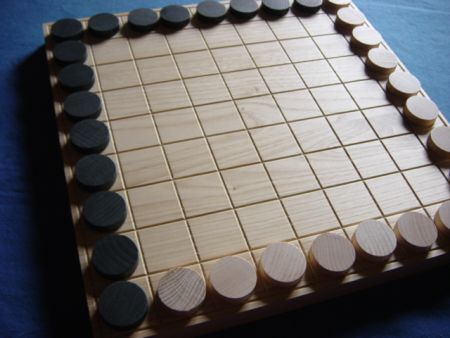
\includegraphics[scale=0.5]{images/mingmang.jpg}
\end{center}
\end{titlepage}
\newpage









\newpage
\begin{center}
\section{Capture des besoins , cahier des charges}
\vspace{2cm}

\subsection{\underline{Résumé:}}
\vspace{1cm}
Il s'agira de développer un jeu de Ming-Mang jouable jusqu'à deux joueurs en console avec Python 3.X , le jeu de ming-mang se pratique sur un plateau de go tibétain et 19x19 et s'apparente au Reversi .Chaque joueur occupe deux bords adjacents du plateau et déplace une pièce en longueur ou en largeur par tour .le jeu se termine si l'un des deux joueurs n'a plus de pions ou si l'un  des deux joueurs n'a plus de pions.

\end{center}

\subsection{\underline{Fonctionnalités:}}
\paragraph{}
Le jeu devra fonctionner en console selon les régles suivantes:
\newline
Les joueurs jouent tour à tour une seule pierre. Les pièces bougent en ligne droite comme
la tour aux échecs. Il n’est pas permis de traverser ou de s’arrêter sur une autre pièce
\newline
\newline
Un joueur ne peut pas jouer un coup qui le ramènerait dans une situation antérieure.
Il peut par contre passer son tour.
\newline
\newline
Toutes pierres encadrées sur une ligne ou une colonne par deux pierres ennemies sont
capturées et remplacées par les pierres de l’adverse
\newline
On ne perd pas sa pièce si on la déplace entre deux adversaires 
\newline
\newline
La partie est finie si un joueur n’a plus de pièces ou si les deux joueurs passent successivement
leur tour.
\newline
\newline
On définit le territoire d’un joueur comme étant la zone du terrain à laquelle il a accès
mais qui ne peut pas être atteinte par son adversaire. Si un joueur possède plus de la
moitié du plateau il gagne automatiquement la partie.
\newline
Dans le cas où les deux joueurs passent leur tour, le joueur ayant plus grand territoire
remporte la partie.
\newline
\newline
Pour jouer , le joueur entre la coordonnée d'un pion a déplacer puis la coordonnée de la case cible , si l'une des règles ci-dessus n'est pas respectée , le programme demandera au joueur de taper de nouvelles coordonnées.

\subsection{\underline{Fonctionnalités additionnelles :}}
\paragraph{}
\begin{center}
\emph{les fonctionnalités ci-dessous seront étudiées mais ne sont pas garanties }
\end{center}
\begin{itemize}
\item Plusieurs variantes de jeu (taille du plateau)
\item Un éditeur de plateau pour créer vos propre terrain de jeu
\item Un mode de jeu joueur contre IA
\item Un mode de jeu joueur contre joueur en réseau local (deux machines connectée sur le meme réseau)
\item Un systéme de sauvegarde et de chargement de partie
\end{itemize}


\subsection{\underline{Priorité , importance relative des fonctionnalités:}}
\paragraph{}
Aucune des fonctionnalités additionnelles listés ci-dessus ne sera intégrée tant que le jeu ne fonctionnera complètement en mode console (déplacement , capture , vérification des règles)

\subsection{\underline{Accessibilité et pré-requis système:}}
\paragraph{}
Pour exécuter le programme , l'utilisateur devra installer Python 3 .Aucun autre module n'est nécessaire pour jouer .Le programme fonctionnera sur la plupart des OS .
\newline
Le jeu est a la porté de n'importe quel utilisateur ayant lu au préalable le manuel d'utilisation


\subsection{\underline{Internationalité:}}
\paragraph{}
Le jeu sera disponible uniquement en Français

\subsection{\underline{Date fixées:}}
\paragraph{}
Le programme , le manuel d'utilisation , le rapport et la documentation HTML seront remis Lundi 25/04/2016

\subsection{\underline{Gestion des erreurs:}}
\paragraph{}
La plupart des entrées utilisateur seront vérifiées et ne pourront pas provoquer d'erreurs. cependant il est possible que si l'utilisateur entre des coordonnées ou des commandes non prévues , le programme plante
\newpage
\begin{center}
\section{Analyse du découpage et de la conception}
\vspace{1cm}
\end{center}
\subsection{\underline{Modules }}
\paragraph{}
Le programme est décomposé en 7 modules différents :
\begin{itemize}
\item Le module main , a partir duquel on lance le programme .Ce module est léger est coordonne le lancement de toutes les autres fonctions
\item Le module gui ; interface avec l'utilisateur , toutes les communications homme-programme passe par ce module .Celui-ci s'avérera utile pour une éventuelle implantation d'interface graphique a l'avenir
\item Le module affiche , dessine la grille a l'initialisation et l'affiche a chaque fin de tour .
\item Le module déplacement , module le plus lourd du programme : Il contient toutes les fonctions d'applications  des choix de l'utilisateur pour tout les mode de jeu ainsi que la vérification des règles.
\item Le module IA , génère une paire de coordonnées pour le mode joueur contre IA basée sur une succession de raisonnement et de règles simple.
\item Modules serveur et client , module du mode de jeu joueur contre joueur en réseau (hélas non fonctionnel), leurs fonctionnement sera expliqué plus loin dans ce rapport
\end{itemize}
\vspace{1cm}
\subsection{\underline{Fonctions du module déplacement }}
\paragraph{}
Le module déplacement est le principal module du programme , il gère les modifications du plateau , ainsi que la vérification du respect des règles :
\newline Lorsque le joueur lance le programme il choisit un mode de jeu , ce choix définira laquelle des trois fonctions de jeu se lance dans le module déplacement (jcia pour le mode de jeu joueur contre ia, jcj pour le mode de jeu classique, ou jcjr pour le mode de jeu en réseau). 
\newline
Une fois le jeu initié les règles sont vérifiées a chaque fois qu'un joueur joue grâce a trois fonctions : la fonctions verifdéplacement qui vérifie les règles de bases tels que l'interdiction du chevauchement des pions ou encore le fait que l'on ne puisse déplacer son pion qu'en colonne ou en ligne .La fonction verifzone vérifie tout les règles liées au principe de territoire et la fonction veriftour qui stoppe le jeu si deux joueurs passent leurs tours.
\newpage
\begin{center}
\section{Fonctionnalités additionnelles}
\end{center}
\paragraph{}
Sur les 5 fonctionnalités additionnelles évoquées dans le cahier des charges , 4 sont opérationnelles dans la version du programme rendue le 25/04 , le mode joueur contre joueur en réseau n'est hélas pas fonctionnel mais les traces de recherche sont toujours présente dans le dossier src du projet.

\subsection{Variantes de plateau}
\paragraph{}
Au lancement l'utilisateur choisis parmi trois variantes de jeu , il s'agit de deux versions de taille différente du plateau classique , Je ne propose pas de plateau a motifs différent car ceux-ci aurait provoqué des problèmes de compatibilité avec le mode IA .En effet celui-ci se base ,entre autre , sur la position initiale des pions pour jouer un coup.

\subsection{Éditeur de plateau}
\paragraph{}
En plus des deux variantes proposées au joueur , celui-ci peut également créer sont propre plateau grâce a l'éditeur de plateau : le joueur choisis la dimension de son plateau puis place un par un les pions .Aucune limite ne lui est imposé , l'utilisateur lance le jeu en tapant "jeu" lorsqu'il a terminé l'édition de son plateau pour lancer la partie , le plateau personnalisé est détruit a la fin de la partie.Pour les mêmes raison évoquées dans le paragraphe précédent , le mode IA n'est pas compatible avec un plateau personnalisé

\subsection{Sauvegarde de partie}
\paragraph{}
En plus d'être très utile  pour tester le programme et corriger les erreurs , la fonction de sauvegarde/chargement de partie est une fonctionnalité simple a implémenter et est donc rentable en terme de temps et d'efforts , celle-ci se base sur le module pickle et permet au joueur de sauvegarder une partie au moment ou il lui est demandé quel pion il souhaite déplacer .Il pourra ensuite retrouver sa partie et rejouer en respectant le tour du joueur au moment il a sauvegarder la partie.

\subsection{IA}
\paragraph{}
Le mode joueur contre IA est la fonctionnalité ayant demandé le plus de travail dans le développement de l'application , elle se base sur un raisonnement simple : durant un certains nombre de tour (varie en fonction de la taille du plateau), l'IA déplace ses pions sur le plateau de manière aléatoire pour permettre de créer des opportunités , puis elle détecte ensuite si elle peut capturer des pions adverses ou défendre ses pions. En fonction du choix le plus intéressant ,elle déplace son pion .Si aucune des deux options n'est possible ou rentable , l'IA déplace un pion au hasard.

\subsection{Joueur contre joueur en réseau local(non fonctionnel)}
\paragraph{}
Le mode joueur contre joueur en réseau local aurait permit a deux joueur de jouer une partie sur deux machines différents .Grâce au module socket , le second joueur n'aurait eu besoin que de télécharger le module client du programme pour pouvoir voir la grille et jouer tout comme son adversaire .
\paragraph{}
Le fonctionnement est le suivant : le joueur hôte lance le programme et choisis le mode joueur contre joueur en réseau .Lorsque que viens le tour du second joueur la fonction jcjr du module déplacement envoie une requête au module serveur qui entre en mode "écoute" , mode dans lequel il attend la connexion d'un client .
\newline
Le module client quand a lui envoie en permanence une demande de connexion a l'IP du module serveur (l'IP est modifiable),lorsque le module client est connecté au module serveur , le module client récupère la grille , l'affiche , et demande le pion a déplacer au second joueur .Une fois les coordonnées entrées le module client les envoies au module serveur qui lui-même les envoie au module déplacement pour qu'il modifie le plateau , la connexion est ensuite fermée par le serveur.
\newline le développement de cette fonctionnalité a été abandonnée faute de temps , les modules client et serveur sont cependant toujours disponible dans le fichier src.
\newpage
\begin{center}
\section{Difficultés rencontrés}
\end{center}

\paragraph{Fonction anti-chevauchement}
La fonction vérifiant que le déplacement commandé par un joueur n'implique pas le chevauchement de deux pions fut la première fonction véritablement compliqué du programme , elle demandait une bonne visualisation de la grille pour bien rédiger les fonctions de parcours .Il s'agit de la fonctionnalité m'ayant demandé le plus de temps et d'essais parmis toutes les autres .Cependant les difficultés que son développement m'a donné m'ont permis de rédiger plus rapidement d'autres fonctions comme la vérification des zones ou la logique de l'IA.
\newline
\newline
\paragraph{Mode joueur contre IA}
Le développement du mode joueur contre IA a été abandonné peu avant la date limite faute de temps , il me fallait me concentrer sur d'autres fonctionnalités plus importantes .

\newpage
\begin{center}
\section{Tests effectués}
\end{center}

\paragraph{}
Une batterie de tests ont été effectués via la fonction assert() de python pour vérifier la fonctionnalité du programme:
\newline

\emph{fonction creegrille(cree le plateau)}
\begin{itemize}
\item test unitaire aux extrêmes : 0 , 999999999 -> fonctionnel
\item test unitaire avec float   : 0.5 0.75  -> erreur si le total de la surface du plateau n'est pas rond
\item test unitaire avec string  : "abs"  -> erreur
\newline
\end{itemize}

\emph{fonction entrecoord(entree des coordonnées )}
\begin{itemize}
\item test unitaire aux extrêmes :  999999999 -> erreur si sortie de la liste g
\item test unitaire avec float   : 0.5 0.75  -> erreur 
\item test unitaire avec string  : "abs"  -> erreur
\end{itemize}

\emph{fonction editplateau(editeur de plateau libre)}
\begin{itemize}
\item test unitaire aux extrêmes pour la couleur du pion: 999999999 -> erreur dans les vérifications de déplacement plus loin dans le programme
\item test unitaire avec float pour la couleur du pion: erreur
\item test unitaire avec string  : "abs"  -> erreur
\item test unitaire aux extrêmes pour les coordonées de placement: 9999999-> erreur si sortie de la grille
\item test unitaire avec float pour les coordonnées: erreur
\item test unitaire avec string pour les coordonnées: erreur
\newline
\end{itemize}


\emph{choixmode(choix du mode de jeu)}
\begin{itemize}
\i



































































\end{document}



